% LaTeX source for ``Think Go: How to Think Like a Computer Scientist''
% Copyright (c)  2015  Allen B. Downey.
% Copyright (c)  2018  Luciano Ramalho.

% License: Creative Commons Attribution-NonCommercial 4.0 Unported License.
% http://creativecommons.org/licenses/by-nc/4.0/
%

%\documentclass[10pt,b5paper]{book}
\documentclass[10pt]{book}
\usepackage[width=5.5in,height=8.5in,hmarginratio=3:2,vmarginratio=1:1]{geometry}

% for some of these packages, you might have to install
% texlive-latex-extra (in Ubuntu)

\usepackage[T1]{fontenc}
\usepackage{textcomp}
\usepackage{mathpazo}
\usepackage{url}
\usepackage{fancyhdr}
\usepackage{graphicx}
\usepackage{amsmath}
\usepackage{amsthm}
%\usepackage{amssymb}
\usepackage{exercise}                        % texlive-latex-extra
\usepackage{makeidx}
\usepackage{setspace}
\usepackage{hevea}                           
\usepackage{upquote}
\usepackage{appendix}
\usepackage[bookmarks]{hyperref}

\title{Think Go}
\author{Allen B. Downey, Chris Mayfield, Luciano Ramalho}
\newcommand{\thetitle}{Think Go: How to Think Like a Computer Scientist}
\newcommand{\theversion}{1st Edition, Version 0.0.0}
\newcommand{\thedate}{}

% these styles get translated in CSS for the HTML version
\newstyle{a:link}{color:black;}
\newstyle{p+p}{margin-top:1em;margin-bottom:1em}
\newstyle{img}{border:0px}

% change the arrows
\setlinkstext
  {\imgsrc[ALT="Previous"]{back.png}}
  {\imgsrc[ALT="Up"]{up.png}}
  {\imgsrc[ALT="Next"]{next.png}}

\makeindex

\newif\ifplastex
\plastexfalse

%%% LR: BEGIN additions for Think Go
\usepackage[utf8]{inputenc}
\usepackage{listings}
\usepackage{listings-golang} % import this package after listings
\usepackage{color}
\usepackage{inconsolata}


% morekeywords=[1]{%keywords: break,case,chan,const,continue,default...
\definecolor{keywordcolor}{rgb}{0,0,0.4}   % blue

% morekeywords=[2]{%built-in func: append,cap,close,complex,copy,delete...
\definecolor{bifcolor}{rgb}{0,0,0.8}     % dark blue

% morekeywords=[3]{%built-in types: bool,byte,complex64,error,float32...
\definecolor{typecolor}{rgb}{0,0,0.8}    % dark blue

% morekeywords=[4]{%predeclared: true,false,iota,nil
\definecolor{constcolor}{rgb}{0.5,0,0.5}    % dark purple

\definecolor{commentcolor}{rgb}{0.4,0.4,0.4}  % gray

\definecolor{stringcolor}{rgb}{0,0.5,0}  % dark green

\lstset{ % add your own preferences
  tabsize=2,
  basicstyle=\small\ttfamily,
  keywordstyle=\color{keywordcolor}\textbf,
  keywordstyle=[2]{\color{bifcolor}\textbf},
  keywordstyle=[3]{\color{typecolor}},
  keywordstyle=[4]{\color{constcolor}\textbf},
  commentstyle=\color{commentcolor},
  stringstyle=\color{stringcolor},
  showstringspaces=false, 
  caption=\lstname,
  captionpos=t, 
  inputpath=code,
  language=Golang
}


%%% LR: END OF additions for Think Go


\begin{document}

\frontmatter

% PLASTEX ONLY
\ifplastex
    \usepackage{localdef}
    \maketitle

\newcount\anchorcnt
\newcommand*{\Anchor}[1]{%
  \@bsphack%
    \Hy@GlobalStepCount\anchorcnt%
    \edef\@currentHref{anchor.\the\anchorcnt}% 
    \Hy@raisedlink{\hyper@anchorstart{\@currentHref}\hyper@anchorend}% 
    \M@gettitle{}\label{#1}% 
    \@esphack%
}


\else
% skip the following for plastex

\newtheorem{exercise}{Exercise}[chapter]

% LATEXONLY

\sloppy
%\setlength{\topmargin}{-0.375in}
%\setlength{\oddsidemargin}{0.0in}
%\setlength{\evensidemargin}{0.0in}

% Uncomment these to center on 8.5 x 11
%\setlength{\topmargin}{0.625in}
%\setlength{\oddsidemargin}{0.875in}
%\setlength{\evensidemargin}{0.875in}

%\setlength{\textheight}{7.2in}

\setlength{\headsep}{3ex}
\setlength{\parindent}{0.0in}
\setlength{\parskip}{1.7ex plus 0.5ex minus 0.5ex}
\renewcommand{\baselinestretch}{1.02}

% see LaTeX Companion page 62
\setlength{\topsep}{-0.0\parskip}
\setlength{\partopsep}{-0.5\parskip}
\setlength{\itemindent}{0.0in}
\setlength{\listparindent}{0.0in}

% see LaTeX Companion page 26
% these are copied from /usr/local/teTeX/share/texmf/tex/latex/base/book.cls
% all I changed is afterskip

\makeatletter

\renewcommand{\section}{\@startsection 
    {section} {1} {0mm}%
    {-3.5ex \@plus -1ex \@minus -.2ex}%
    {0.7ex \@plus.2ex}%
    {\normalfont\Large\bfseries}}
\renewcommand\subsection{\@startsection {subsection}{2}{0mm}%
    {-3.25ex\@plus -1ex \@minus -.2ex}%
    {0.3ex \@plus .2ex}%
    {\normalfont\large\bfseries}}
\renewcommand\subsubsection{\@startsection {subsubsection}{3}{0mm}%
    {-3.25ex\@plus -1ex \@minus -.2ex}%
    {0.3ex \@plus .2ex}%
    {\normalfont\normalsize\bfseries}}

% The following line adds a little extra space to the column
% in which the Section numbers appear in the table of contents
\renewcommand{\l@section}{\@dottedtocline{1}{1.5em}{3.0em}}
\setcounter{tocdepth}{1}

\makeatother

\newcommand{\beforefig}{\vspace{1.3\parskip}}
\newcommand{\afterfig}{\vspace{-0.2\parskip}}

\newcommand{\beforeverb}{\vspace{0.6\parskip}}
\newcommand{\afterverb}{\vspace{0.6\parskip}}

\newcommand{\adjustpage}[1]{\enlargethispage{#1\baselineskip}}


% Note: the following command seems to cause problems for Acroreader
% on Windows, so for now I am overriding it.
%\newcommand{\clearemptydoublepage}{
%            \newpage{\pagestyle{empty}\cleardoublepage}}
\newcommand{\clearemptydoublepage}{\cleardoublepage}

%\newcommand{\blankpage}{\pagestyle{empty}\vspace*{1in}\newpage}
\newcommand{\blankpage}{\vspace*{1in}\newpage}

% HEADERS

\renewcommand{\chaptermark}[1]{\markboth{#1}{}}
\renewcommand{\sectionmark}[1]{\markright{\thesection\ #1}{}}

\lhead[\fancyplain{}{\bfseries\thepage}]%
      {\fancyplain{}{\bfseries\rightmark}}
\rhead[\fancyplain{}{\bfseries\leftmark}]%
      {\fancyplain{}{\bfseries\thepage}}
\cfoot{}

\pagestyle{fancyplain}


% turn off the rule under the header
%\setlength{\headrulewidth}{0pt}

% the following is a brute-force way to prevent the headers
% from getting transformed into all-caps
\renewcommand\MakeUppercase{}

% Exercise environment
\newtheoremstyle{myex}% name
     {9pt}%      Space above
     {9pt}%      Space below
     {}%         Body font
     {}%         Indent amount (empty = no indent, \parindent = para indent)
     {\bfseries}% Thm head font
     {}%        Punctuation after thm head
     {0.5em}%     Space after thm head: " " = normal interword space;
           %       \newline = linebreak
     {}%         Thm head spec (can be left empty, meaning `normal')

\theoremstyle{myex}


\begin{latexonly}

\renewcommand{\blankpage}{\thispagestyle{empty} \quad \newpage}

%\blankpage
%\blankpage

% TITLE PAGES FOR LATEX VERSION

%-half title--------------------------------------------------
\thispagestyle{empty}

\begin{flushright}
\vspace*{2.0in}

\begin{spacing}{3}
{\huge Think Go}\\
{\Large How to Think Like a Computer Scientist}
\end{spacing}

\vspace{0.25in}

\theversion

\thedate

\vfill

\end{flushright}

%--verso------------------------------------------------------

\blankpage
\blankpage
%\clearemptydoublepage
%\pagebreak
%\thispagestyle{empty}
%\vspace*{6in}

%--title page--------------------------------------------------
\pagebreak
\thispagestyle{empty}

\begin{flushright}
\vspace*{2.0in}

\begin{spacing}{3}
{\huge Think Go}\\
{\Large How to Think Like a Computer Scientist}
\end{spacing}

\vspace{0.25in}

\theversion

\thedate

\vspace{1in}


{\Large
Allen Downey, Chris Mayfield, Luciano Ramalho\\
}


\vspace{0.5in}

{\Large Green Tea Press}

{\small Needham, Massachusetts}

%\includegraphics[width=1in]{figs/logo1.pdf}
\vfill

\end{flushright}


%--copyright--------------------------------------------------
\pagebreak
\thispagestyle{empty}

{\small
Copyright \copyright ~2015 Allen Downey.

Copyright \copyright ~2018 Luciano Ramalho.


\vspace{0.2in}

\begin{flushleft}
Green Tea Press       \\
9 Washburn Ave        \\
Needham MA 02492
\end{flushleft}

Permission is granted to copy, distribute, and/or modify this document
under the terms of the Creative Commons Attribution-NonCommercial 4.0 Unported
License, which is available at \url{http://creativecommons.org/licenses/by-nc/4.0/}.

The original form of this book is \LaTeX\ source code.  Compiling this
\LaTeX\ source has the effect of generating a device-independent
representation of a textbook, which can be converted to other formats
and printed.

The \LaTeX\ source for this book is available from
\url{https://tgo.li/2DKtewu}

\vspace{0.2in}

} % end small

\end{latexonly}

% HTMLONLY

\begin{htmlonly}

% TITLE PAGE FOR HTML VERSION

{\Large \thetitle}

{\large Allen Downey, Chris Mayfield, Luciano Ramalho}

\theversion

\thedate

\setcounter{chapter}{-1}

\end{htmlonly}

\fi
% END OF THE PART WE SKIP FOR PLASTEX


\chapter{Preface}

\begin{quote}
This book is a work in progress. This {\bf Preface} will be the last chapter written. Please skip to {\bf Chapter 1} to see some progress.  -- LR
\end{quote}

{\it Think Go} is an introduction to computer science and programming intended for readers with little or no experience.
We start with the most basic concepts and are careful to define all terms when they are first used.
The book presents each new idea in a logical progression.
Larger topics, like control flow statements and interfaces, are divided into smaller examples and introduced over the course of several chapters.

\section*{The strange history of this book}

In January 1999 I was preparing to teach an introductory programming
class in Java.  I had taught it three times and I was getting
frustrated.  The failure rate in the class was too high and, even for
students who succeeded, the overall level of achievement was too low.

One of the problems I saw was the books.  
They were too big, with too much unnecessary detail about Java, and
not enough high-level guidance about how to program.  And they all
suffered from the trap door effect: they would start out easy,
proceed gradually, and then somewhere around Chapter 5 the bottom would
fall out.  The students would get too much new material, too fast,
and I would spend the rest of the semester picking up the pieces.

Two weeks before the first day of classes, I decided to write my
own book.  My goals were:

\begin{itemize}

\item Keep it short.  It is better for students to read 10 pages
than not read 50 pages.

\item Be careful with vocabulary.  I tried to minimize jargon
and define each term at first use.

\item Build gradually. To avoid trap doors, I took the most difficult
topics and split them into a series of small steps. 

\item Focus on programming, not the programming language.  I included
the minimum useful subset of Java and left out the rest.

\end{itemize}

I needed a title, so on a whim I chose {\em How to Think Like
a Computer Scientist}.

My first version was rough, but it worked.  Students did the reading,
and they understood enough that I could spend class time on the hard
topics, the interesting topics and (most important) letting the
students practice.

I released the book under the GNU Free Documentation License,
which allows users to copy, modify, and distribute the book.
\index{GNU Free Documentation License}
\index{Free Documentation License, GNU}

What happened next is the cool part.  Jeff Elkner, a high school
teacher in Virginia, adopted my book and translated it into
Python.  He sent me a copy of his translation, and I had the
unusual experience of learning Python by reading my own book.
As Green Tea Press, I published the first Python version in 2001.
\index{Elkner, Jeff}

In 2003 I started teaching at Olin College and I got to teach
Python for the first time.  The contrast with Java was striking.
Students struggled less, learned more, worked on more interesting
projects, and generally had a lot more fun.
\index{Olin College}

Since then I've continued to develop the book,
correcting errors, improving some of the examples and
adding material, especially exercises.

The result is this book, now with the less grandiose title
{\em Think Python}.  Some of the changes are:

\begin{itemize}

\item I added a section about debugging at the end of each chapter.
  These sections present general techniques for finding and avoiding
  bugs, and warnings about Python pitfalls.

\item I added more exercises, ranging from short tests of
  understanding to a few substantial projects.  Most exercises
  include a link to my solution.

\item I added a series of case studies---longer examples with
  exercises, solutions, and discussion.
  
\item I expanded the discussion of program development plans
  and basic design patterns.

\item I added appendices about debugging and analysis of algorithms.

\end{itemize}

The second edition of {\em Think Python} has these new features:

\begin{itemize}

\item The book and all supporting code have been updated to Python 3.

\item I added a few sections, and more details on the web, to help
beginners get started running Python in a browser, so you don't have
to deal with installing Python until you want to.

\item For Chapter~\ref{turtle} I switched from my own turtle graphics
  package, called Swampy, to a more standard Python module, {\tt
    turtle}, which is easier to install and more powerful.

\item I added a new chapter called ``The Goodies'', which introduces
some additional Python features that are not strictly necessary, but
sometimes handy.

\end{itemize}

I hope you enjoy working with this book, and that it helps
you learn to program and think like
a computer scientist, at least a little bit.


Allen B. Downey \\

Olin College \\


\section*{Acknowledgments}

Many thanks to Jeff Elkner, who
translated my Java book into Python, which got this project
started and introduced me to what has turned out to be my
favorite language.
\index{Elkner, Jeff}

Thanks also to Chris Meyers, who contributed several sections
to {\em How to Think Like a Computer Scientist}.
\index{Meyers, Chris}

Thanks to the Free Software Foundation for developing
the GNU Free Documentation License, which helped make
my collaboration with Jeff and Chris possible, and Creative
Commons for the license I am using now.
\index{GNU Free Documentation License}
\index{Free Documentation License, GNU}
\index{Creative Commons}

Thanks to the editors at Lulu who worked on
{\em How to Think Like a Computer Scientist}.

Thanks to the editors at O'Reilly Media who worked on
{\em Think Python}.

Thanks to all the students who worked with earlier
versions of this book and all the contributors (listed
below) who sent in corrections and suggestions.


\section*{Contributor List}

\index{contributors}
More than 100 sharp-eyed and thoughtful readers have sent in
suggestions and corrections over the past few years.  Their
contributions, and enthusiasm for this project, have been a
huge help.

If you have a suggestion or correction, please send email to 
{\tt feedback@thinkpython.com}.  If I make a change based on your
feedback, I will add you to the contributor list
(unless you ask to be omitted).

If you include at least part of the sentence the
error appears in, that makes it easy for me to search.  Page and
section numbers are fine, too, but not quite as easy to work with.
Thanks!

\begin{itemize}

\small
\item Lloyd Hugh Allen sent in a correction to Section 8.4.

\item Yvon Boulianne sent in a correction of a semantic error in
Chapter 5.

\item Fred Bremmer submitted a correction in Section 2.1.

\item Jonah Cohen wrote the Perl scripts to convert the
LaTeX source for this book into beautiful HTML.

\item Michael Conlon sent in a grammar correction in Chapter 2
and an improvement in style in Chapter 1, and he initiated discussion
on the technical aspects of interpreters.

\item Benoit Girard sent in a
correction to a humorous mistake in Section 5.6.

\item Courtney Gleason and Katherine Smith wrote {\tt horsebet.py},
which was used as a case study in an earlier version of the book.  Their
program can now be found on the website.

\item Lee Harr submitted more corrections than we have room to list
here, and indeed he should be listed as one of the principal editors
of the text.

\item James Kaylin is a student using the text. He has submitted
numerous corrections.

\item David Kershaw fixed the broken {\tt catTwice} function in Section
3.10.

\item Eddie Lam has sent in numerous corrections to Chapters 
1, 2, and 3.
He also fixed the Makefile so that it creates an index the first time it is
run and helped us set up a versioning scheme.  

\item Man-Yong Lee sent in a correction to the example code in
Section 2.4.  

\item David Mayo pointed out that the word ``unconsciously"
in Chapter 1 needed
to be changed to ``subconsciously".

\item Chris McAloon sent in several corrections to Sections 3.9 and
3.10.

\item Matthew J. Moelter has been a long-time contributor who sent
in numerous corrections and suggestions to the book.  

\item Simon Dicon Montford reported a missing function definition and
several typos in Chapter 3.  He also found errors in the {\tt increment}
function in Chapter 13.

\item John Ouzts corrected the definition of ``return value"
in Chapter 3.

\item Kevin Parks sent in valuable comments and suggestions as to how
to improve the distribution of the book.

\item David Pool sent in a typo in the glossary of Chapter 1, as well
as kind words of encouragement.

\item Michael Schmitt sent in a correction to the chapter on files
and exceptions.

\item Robin Shaw pointed out an error in Section 13.1, where the
printTime function was used in an example without being defined.

\item Paul Sleigh found an error in Chapter 7 and a bug in Jonah Cohen's
Perl script that generates HTML from LaTeX.

\item Craig T. Snydal is testing the text in a course at Drew
University.  He has contributed several valuable suggestions and corrections.

\item Ian Thomas and his students are using the text in a programming
course.  They are the first ones to test the chapters in the latter half
of the book, and they have made numerous corrections and suggestions.

\item Keith Verheyden sent in a correction in Chapter 3.

\item Peter Winstanley let us know about a longstanding error in
our Latin in Chapter 3.

\item Chris Wrobel made corrections to the code in the chapter on
file I/O and exceptions. 

\item Moshe Zadka has made invaluable contributions to this project.
In addition to writing the first draft of the chapter on Dictionaries, he
provided continual guidance in the early stages of the book.

\item Christoph Zwerschke sent several corrections and
pedagogic suggestions, and explained the difference between {\em gleich}
and {\em selbe}.

\item James Mayer sent us a whole slew of spelling and
typographical errors, including two in the contributor list.

\item Hayden McAfee caught a potentially confusing inconsistency
between two examples.

\item Angel Arnal is part of an international team of translators
working on the Spanish version of the text.  He has also found several
errors in the English version.

\item Tauhidul Hoque and Lex Berezhny created the illustrations
in Chapter 1 and improved many of the other illustrations.

\item Dr. Michele Alzetta caught an error in Chapter 8 and sent
some interesting pedagogic comments and suggestions about Fibonacci
and Old Maid.

\item Andy Mitchell caught a typo in Chapter 1 and a broken example
in Chapter 2.

\item Kalin Harvey suggested a clarification in Chapter 7 and
caught some typos.

\item Christopher P. Smith caught several typos and helped us
update the book for Python 2.2.

\item David Hutchins caught a typo in the Foreword.

\item Gregor Lingl is teaching Python at a high school in Vienna,
Austria.  He is working on a German translation of the book,
and he caught a couple of bad errors in Chapter 5.

\item Julie Peters caught a typo in the Preface.

\item Florin Oprina sent in an improvement in {\tt makeTime},
a correction in {\tt printTime}, and a nice typo.

\item D.~J.~Webre suggested a clarification in Chapter 3.

\item Ken found a fistful of errors in Chapters 8, 9 and 11.

\item Ivo Wever caught a typo in Chapter 5 and suggested a clarification
in Chapter 3.

\item Curtis Yanko suggested a clarification in Chapter 2.

\item Ben Logan sent in a number of typos and problems with translating
the book into HTML.

\item Jason Armstrong saw the missing word in Chapter 2.

\item Louis Cordier noticed a spot in Chapter 16 where the code
didn't match the text.

\item Brian Cain suggested several clarifications in Chapters 2 and 3.

\item Rob Black sent in a passel of corrections, including some
changes for Python 2.2.

\item Jean-Philippe Rey at Ecole Centrale
Paris sent a number of patches, including some updates for Python 2.2
and other thoughtful improvements.

\item Jason Mader at George Washington University made a number
of useful suggestions and corrections.

\item Jan Gundtofte-Bruun reminded us that ``a error'' is an error.

\item Abel David and Alexis Dinno reminded us that the plural of
``matrix'' is ``matrices'', not ``matrixes''.  This error was in the
book for years, but two readers with the same initials reported it on
the same day.  Weird.

\item Charles Thayer encouraged us to get rid of the semi-colons
we had put at the ends of some statements and to clean up our
use of ``argument'' and ``parameter''.

\item Roger Sperberg pointed out a twisted piece of logic in Chapter 3.

\item Sam Bull pointed out a confusing paragraph in Chapter 2.

\item Andrew Cheung pointed out two instances of ``use before def''.

\item C. Corey Capel spotted the missing word in the Third Theorem
of Debugging and a typo in Chapter 4.

\item Alessandra helped clear up some Turtle confusion.

\item Wim Champagne found a brain-o in a dictionary example.

\item Douglas Wright pointed out a problem with floor division in
{\tt arc}.

\item Jared Spindor found some jetsam at the end of a sentence.

\item Lin Peiheng sent a number of very helpful suggestions.

\item Ray Hagtvedt sent in two errors and a not-quite-error.

\item Torsten H\"{u}bsch pointed out an inconsistency in Swampy.

\item Inga Petuhhov corrected an example in Chapter 14.

\item Arne Babenhauserheide sent several helpful corrections.

\item Mark E. Casida is is good at spotting repeated words.

\item Scott Tyler filled in a that was missing.  And then sent in
a heap of corrections.

\item Gordon Shephard sent in several corrections, all in separate
emails.

\item Andrew Turner {\tt spot}ted an error in Chapter 8.

\item Adam Hobart fixed a problem with floor division in {\tt arc}.

\item Daryl Hammond and Sarah Zimmerman pointed out that I served
up {\tt math.pi} too early.  And Zim spotted a typo.

\item George Sass found a bug in a Debugging section.

\item Brian Bingham suggested Exercise~\ref{exrotatepairs}.

\item Leah Engelbert-Fenton pointed out that I used {\tt tuple}
as a variable name, contrary to my own advice.  And then found
a bunch of typos and a ``use before def''.

\item Joe Funke spotted a typo.

\item Chao-chao Chen found an inconsistency in the Fibonacci example.

\item Jeff Paine knows the difference between space and spam.

\item Lubos Pintes sent in a typo.

\item Gregg Lind and Abigail Heithoff suggested Exercise~\ref{checksum}.

\item Max Hailperin has sent in a number of corrections and
  suggestions.  Max is one of the authors of the extraordinary {\em
    Concrete Abstractions}, which you might want to read when you are
  done with this book.

\item Chotipat Pornavalai found an error in an error message.

\item Stanislaw Antol sent a list of very helpful suggestions.

\item Eric Pashman sent a number of corrections for Chapters 4--11.

\item Miguel Azevedo found some typos.

\item Jianhua Liu sent in a long list of corrections.

\item Nick King found a missing word.

\item Martin Zuther sent a long list of suggestions.

\item Adam Zimmerman found an inconsistency in my instance
of an ``instance'' and several other errors.

\item Ratnakar Tiwari suggested a footnote explaining degenerate
triangles.

\item Anurag Goel suggested another solution for \verb"is_abecedarian"
and sent some additional corrections.  And he knows how to
spell Jane Austen.

\item Kelli Kratzer spotted one of the typos.

\item Mark Griffiths pointed out a confusing example in Chapter 3.

\item Roydan Ongie found an error in my Newton's method.

\item Patryk Wolowiec helped me with a problem in the HTML version.

\item Mark Chonofsky told me about a new keyword in Python 3.

\item Russell Coleman helped me with my geometry.

\item Nam Nguyen found a typo and pointed out that I used the Decorator
pattern but didn't mention it by name.

\item St\'{e}phane Morin sent in several corrections and suggestions.

\item Paul Stoop corrected a typo in \verb+uses_only+.

\item Eric Bronner pointed out a confusion in the discussion of the
order of operations.

\item Alexandros Gezerlis set a new standard for the number and
quality of suggestions he submitted.  We are deeply grateful!

\item Gray Thomas knows his right from his left.

\item Giovanni Escobar Sosa sent a long list of corrections and
suggestions.

\item Daniel Neilson corrected an error about the order of operations.

\item Will McGinnis pointed out that {\tt polyline} was defined
differently in two places.

\item Frank Hecker pointed out an exercise that was under-specified, and
some broken links.

\item Animesh B helped me clean up a confusing example.

\item Martin Caspersen found two round-off errors.

\item Gregor Ulm sent several corrections and suggestions.

\item Dimitrios Tsirigkas suggested I clarify an exercise.

\item Carlos Tafur sent a page of corrections and suggestions.

\item Martin Nordsletten found a bug in an exercise solution.

\item Sven Hoexter pointed out that a variable named {\tt input}
shadows a build-in function.

\item Stephen Gregory pointed out the problem with {\tt cmp}
in Python 3.

\item Ishwar Bhat corrected my statement of Fermat's last theorem.

\item Andrea Zanella translated the book into Italian, and sent a
number of corrections along the way.

\item Many, many thanks to Melissa Lewis and Luciano Ramalho for
  excellent comments and suggestions on the second edition.

\item Thanks to Harry Percival from PythonAnywhere for his help
getting people started running Python in a browser.

\item Xavier Van Aubel made several useful corrections in the second
edition.

\item William Murray corrected my definition of floor division.

\item Per Starb{\"a}ck brought me up to date on universal newlines in Python 3. 

% ENDCONTRIB

In addition, people who spotted typos or made corrections include
Czeslaw Czapla, Dale Wilson,
Richard Fursa, Brian McGhie, Lokesh Kumar Makani, Matthew Shultz, Viet
Le, Victor Simeone, Lars O.D. Christensen, Swarup Sahoo, Alix Etienne,
Kuang He, Wei Huang, Karen Barber, and Eric Ransom.


\end{itemize}


\normalsize
\clearemptydoublepage

% TABLE OF CONTENTS
\begin{latexonly}

\tableofcontents

\clearemptydoublepage

\end{latexonly}



% START THE BOOK
\mainmatter


\chapter{The way of the program}

The goal of this book is to teach you to think like a computer scientist. This
way of thinking combines some of the best features of mathematics,
engineering, and natural science. Like mathematicians, computer scientists use
formal languages to denote ideas (specifically computations). Like engineers,
they design things, assembling components into systems and evaluating
tradeoffs among alternatives. Like scientists, they observe the behavior of
complex systems, form hypotheses, and test predictions. \index{problem
solving}

The single most important skill for a computer scientist is {\bf problem
solving}. Problem solving means the ability to formulate problems, think
creatively about solutions, and express a solution clearly and accurately. As
it turns out, the process of learning to program is an excellent opportunity
to practice problem-solving skills. That's why this chapter is called, ``The
way of the program''.

On one level, you will be learning to program, a useful skill by itself. On
another level, you will use programming as a means to an end. As we go along,
that end will become clearer.


\section{What is a program?}

A {\bf program} is a sequence of instructions that specifies how to perform a
computation. The computation might be something mathematical, such as solving
a system of equations or finding the roots of a polynomial, but it can also be
a symbolic computation, such as searching and replacing text in a document or
something graphical, like processing an image or playing a video.
\index{program}

The details look different in different languages, but a few basic
instructions appear in just about every language:

\begin{description}

\item[input:] Get data from the keyboard, a file, the network,  a camera, or
some other device like a fingerprint reader.

\item[output:] Display data on the screen, save it in a file, send it over the
network, or control a device such as a door lock.

\item[math:] Perform basic mathematical operations like addition and
multiplication.

\item[decisions:] Check for certain conditions to determine whether to perform
some action. For example: if the fingerprint matches, unlock the door.

\item[repetition:] Perform some action repeatedly, usually with some
variation.

\end{description}

Believe it or not, that's pretty much all there is to it. Every program you've
ever used, no matter how complicated, is made up of instructions that look
pretty much like these. So you can think of programming as the process of
breaking a large, complex task into smaller and smaller subtasks until the
subtasks are simple enough to be performed with one of these basic
instructions.


\section{Running Go}
\index{Go!running}

One of the challenges of getting started with Go is that you might have to
install Go and related software on your computer. If you are familiar with
your operating system, and especially if you are comfortable with the command-
line interface, you will have no trouble installing Go. But for beginners, it
can be distracting to learn about system administration and programming at the
same time.

To avoid that problem, we recommend that you start out using the
{\it Go Playground}:
\index{Go Playground}

\url{https://play.golang.org/}

The {\it Go Playground} lets you type or paste Go code and click a button
to run it, without installing anything. It is limited in many ways, but good
enough to get started. After you've taken the first steps, we'll provide
instructions for installing Go on your computer.\footnote{If you can't wait to
install Go, Appendix A explains how.}


\section{The hello world program}
\label{hello}

Traditionally, the first program you write when learning a new programming
language is called the hello world program. All it does is display the
words ``Hello, World!''\ on the screen.
In Go, it looks like this:

\index{hello.go}
\lstinputlisting[language=Golang,label=lst:hello.go]{01/hello/hello.go}

We typed listing \ref{lst:hello.go} and saved it in the playground.
Follow this link to see it:

\url{https://tgo.li/2r8yCXj}

If you open that address in a browser, you'll see a page similar to Figure~\ref{fig:playhello}.

\begin{figure}[!ht]
\begin{center}
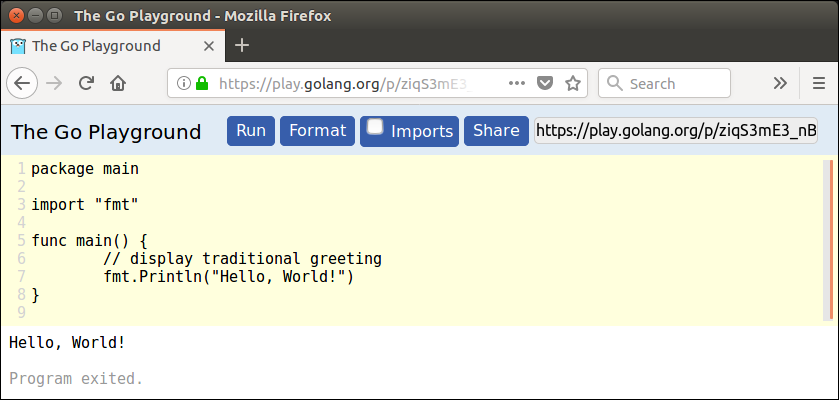
\includegraphics[width=1.0\textwidth]{figs/play-hello.png}
\caption{The hello world program in the Go playground (after running).}
\label{fig:playhello}
\end{center}
\end{figure}

To execute the program, click the blue button labeled {\bf Run}. You may
briefly see the message {\tt Waiting for remote server...}, and then the
output will appear below the code listing, as pictured. Note that the output
does not include the quotation marks around ``Hello, World!''\ .

We want invite you to try editing the hello world program, but we need words
to describe parts of a program so we can talk about it. The next section
covers some basic terms.


\section{Program structure}
\label{program structure}

Go programs are made up of {\bf declarations}. In listing \ref{lst:hello.go}
we have three declarations: {\tt package}, {\tt import}, and {\tt func}.

We'll have a lot more to say about those declarations, but basically this is
what they mean, starting with the most fundamental one, {\tt func}:

\begin{description}

\item[\textbf{\texttt{func}}:] This declares a {\bf function}, which is a
sequence of lines of code that perform some computation or action. The only
function in \ref{lst:hello.go} has the special name {\tt main}. When a Go
program runs, it starts at the first line in the function named {\tt main} and
ends when it executes the last line in it.

\item[\textbf{\texttt{package}}:] All Go code is organized in {\bf packages},
which consist of one or more text files. The package name {\tt main} is
mandatory for stand-alone programs --- as opposed to {\bf library packages}
that are not complete programs, but provide functions for other programs.

\item[\textbf{\texttt{import}}:] This declaration tells Go which library
packages are needed to build our program. Our {\tt main} function uses the
{\tt fmt.Println} function, therefore we need to import {\tt fmt}. The {\tt
fmt} package provides text formatting and output functions.

\end{description}

Programming in Go is writing functions inside packages. Very often, our
functions will use functions from library packages that we import. In this
book we'll mostly write stand-alone programs, but we'll use many libraries
written by others.


\section{Exercises}

\begin{exercise}

It is a good idea to read this book in front of a computer so you can try out
the examples as you go.

Whenever you are experimenting with a new feature, you should try to make
mistakes. 

This kind of experiment helps you remember what you read; it also
helps when you are programming, because you get to know what the error
messages mean. It is better to make mistakes now and on purpose than
later and accidentally.
\index{error message}

Start with {\tt hello.go} and make the changes suggested here. To recover
the original code, just visit that same URL:

\url{https://tgo.li/2r8yCXj}

After each change, hit the {\bf Run} button to see what happens.

\begin{enumerate}

\item What if there is no {\tt package} statement?

\item What if the {\tt package} name is {\tt banana} instead of {\tt main}? 

\item If you are trying to print a string, what happens if you
leave out one of the quotation marks, or both?

\item You can use a minus sign to make a negative number like
{\tt -2}. What happens if you put a plus sign before a number?
What about {\tt 2++2}?

\item In math notation, leading zeros are ok, as in {\tt 02}.
What happens if you try this in Python?

\item What happens if you have two values with no operator
between them?

\end{enumerate}

\end{exercise}


\section{Anatomy of a function}
\label{function!syntax}

Let's take a closer look at the {\tt main} function from \ref{lst:hello.go}:

\begin{lstlisting}
func main() {
	// display traditional greeting
	fmt.Println("Hello, World!")
}
\end{lstlisting}

\index{main}

We try to give descriptive names to functions. The name {\tt main} is not very
descriptive, but it is special as we just saw.

\index{\{\} curly braces}
\index{brackets!curly}

Go uses curly braces (\{ and \}) to group things together. In {\tt main}, the
braces contain the two lines that make up the body of the function. Those
lines are indented from the left margin to make it clear that they are inside
the function declaration.

\index{comment!end-of-line}
\index{statement!comment}

The line that begins with two slashes {\tt //} is a {\bf comment}, which is a
bit of English text that explains the code. When Go sees {\tt //}, it ignores
everything from there until the end of the line. Comments have no effect on
the execution of the program, but they make it easier for other programmers
(and your future self) to understand what you meant to do.

The second line in {\tt main} main is a {\bf statement}, a line of code that
performs a basic action. A common way of performing actions is to call
functions from library packages. So you write functions and your functions, in
turn, call other functions. In the hello world program, this statement calls
the {\tt fmt.Println} function to display a message on the screen:

\begin{lstlisting}
	fmt.Println("Hello, World!")
\end{lstlisting}

The name {\tt Println} stands for ``print line''. Confusingly, in programming,
{\em print} can mean both ``display on the screen'' and ``send to the
printer''. In this book, we'll try to say ``display'' when we mean output to
the screen.

\index{case-sensitive} Go is ``case-sensitive'', which means that uppercase
and lowercase are not the same. In this example, {\tt Println} has to begin
with an uppercase letter; {\tt println} and {\tt PRINTLN} won't work.



There are a number of web pages you can use to run Python. If you
already have a favorite, go ahead and use it. Otherwise I recommend
PythonAnywhere. we provide detailed instructions for getting started
at \url{http://tinyurl.com/thinkpython2e}. 
\index{PythonAnywhere}

There are two versions of Python, called Python 2 and Python 3.
They are very similar, so if you learn one, it is easy to switch
to the other. In fact, there are only a few differences you will
encounter as a beginner.
This book is written for Python 3, but we include some notes
about Python 2.
\index{Python 2}

The Python {\bf interpreter} is a program that reads and executes
Python code. Depending on your environment, you might start the
interpreter by clicking on an icon, or by typing {\tt python} on
a command line. 
When it starts, you should see output like this:
\index{interpreter}

\begin{verbatim}
Python 3.4.0 (default, Jun 19 2015, 14:20:21) 
[GCC 4.8.2] on linux
Type "help", "copyright", "credits" or "license" for more information.
>>> 
\end{verbatim}
%
The first three lines contain information about the interpreter
and the operating system it's running on, so it might be different for
you. But you should check that the version number, which is
{\tt 3.4.0} in this example, begins with 3, which indicates that
you are running Python 3. If it begins with 2, you are running
(you guessed it) Python 2.

The last line is a {\bf prompt} that indicates that the interpreter is
ready for you to enter code.
If you type a line of code and hit Enter, the interpreter displays the
result: 
\index{prompt}

\begin{verbatim}
>>> 1 + 1
2
\end{verbatim}
%
Now you're ready to get started.
From here on, we assume that you know how to start the Python
interpreter and run code.


\section{The first program}
\label{hello}
\index{Hello, World}

Traditionally, the first program you write in a new language
is called ``Hello, World!'' because all it does is display the
words ``Hello, World!''. In Python, it looks like this:

\begin{verbatim}
>>> print('Hello, World!')
\end{verbatim}
%
This is an example of a {\bf print statement}, although it
doesn't actually print anything on paper. It displays a result on the
screen. In this case, the result is the words

\begin{verbatim}
Hello, World!
\end{verbatim}
%
The quotation marks in the program mark the beginning and end
of the text to be displayed; they don't appear in the result.
\index{quotation mark}
\index{print statement}
\index{statement!print}

The parentheses indicate that {\tt print} is a function. We'll get
to functions in Chapter~\ref{funcchap}.
\index{function} \index{print function}

In Python 2, the print statement is slightly different; it is not
a function, so it doesn't use parentheses.
\index{Python 2}

\begin{verbatim}
>>> print 'Hello, World!'
\end{verbatim}
%
This distinction will make more sense soon, but that's enough to
get started.


\section{Arithmetic operators}
\index{operator!arithmetic}
\index{arithmetic operator}

After ``Hello, World'', the next step is arithmetic. Python provides
{\bf operators}, which are special symbols that represent computations
like addition and multiplication. 

The operators {\tt +}, {\tt -}, and {\tt *} perform addition,
subtraction, and multiplication, as in the following examples:

\begin{verbatim}
>>> 40 + 2
42
>>> 43 - 1
42
>>> 6 * 7
42
\end{verbatim}
%
The operator {\tt /} performs division:

\begin{verbatim}
>>> 84 / 2
42.0
\end{verbatim}
%
You might wonder why the result is {\tt 42.0} instead of {\tt 42}.
we'll explain in the next section.

Finally, the operator {\tt **} performs exponentiation; that is,
it raises a number to a power:

\begin{verbatim}
>>> 6**2 + 6
42
\end{verbatim}
%
In some other languages, \verb"^" is used for exponentiation, but
in Python it is a bitwise operator called XOR. If you are not
familiar with bitwise operators, the result will surprise you:

\begin{verbatim}
>>> 6 ^ 2
4
\end{verbatim}
%
we won't cover
bitwise operators in this book, but you can read about
them at \url{http://wiki.python.org/moin/BitwiseOperators}.
\index{bitwise operator}
\index{operator!bitwise}


\section{Values and types}
\index{value}
\index{type}
\index{string}

A {\bf value} is one of the basic things a program works with, like a
letter or a number. Some values we have seen so far are {\tt 2},
{\tt 42.0}, and \verb"'Hello, World!'".

These values belong to different {\bf types}:
{\tt 2} is an {\bf integer}, {\tt 42.0} is a {\bf floating-point number},
and \verb"'Hello, World!'" is a {\bf string},
so-called because the letters it contains are strung together.
\index{integer}
\index{floating-point}

If you are not sure what type a value has, the interpreter can
tell you:

\begin{verbatim}
>>> type(2)
<class 'int'>
>>> type(42.0)
<class 'float'>
>>> type('Hello, World!')
<class 'str'>
\end{verbatim}
%
In these results, the word ``class'' is used in the sense of
a category; a type is a category of values.
\index{class}

Not surprisingly, integers belong to the type {\tt int},
strings belong to {\tt str} and floating-point
numbers belong to {\tt float}. 
\index{type}
\index{string type}
\index{type!str}
\index{int type}
\index{type!int}
\index{float type}
\index{type!float}

What about values like \verb"'2'" and \verb"'42.0'"?
They look like numbers, but they are in quotation marks like
strings.
\index{quotation mark}

\begin{verbatim}
>>> type('2')
<class 'str'>
>>> type('42.0')
<class 'str'>
\end{verbatim}
%
They're strings.

When you type a large integer, you might be tempted to use commas
between groups of digits, as in {\tt 1,000,000}. This is not a
legal {\em integer} in Python, but it is legal:

\begin{verbatim}
>>> 1,000,000
(1, 0, 0)
\end{verbatim}
%
That's not what we expected at all!  Python interprets {\tt
  1,000,000} as a comma-separated sequence of integers. We'll learn
more about this kind of sequence later.
\index{sequence}

%This is the first example we have seen of a semantic error: the code
%runs without producing an error message, but it doesn't do the
%``right'' thing.
%\index{semantic error}
%\index{error!semantic}
%\index{error message}
% TODO: use this as an example of a semantic error later



\section{Formal and natural languages}
\index{formal language}
\index{natural language}
\index{language!formal}
\index{language!natural}

{\bf Natural languages} are the languages people speak,
such as English, Spanish, and French. They were not designed
by people (although people try to impose some order on them);
they evolved naturally.

{\bf Formal languages} are languages that are designed by people for
specific applications. For example, the notation that mathematicians
use is a formal language that is particularly good at denoting
relationships among numbers and symbols. Chemists use a formal
language to represent the chemical structure of molecules. And
most importantly:

\begin{quote}
{\bf Programming languages are formal languages that have been
designed to express computations.}
\end{quote}

Formal languages tend to have strict {\bf syntax} rules that
govern the structure of statements.
For example, in mathematics the statement
$3 + 3 = 6$ has correct syntax, but
$3 + = 3 \$ 6$ does not. In chemistry
$H_2O$ is a syntactically correct formula, but $_2Zz$ is not.
\index{syntax}

Syntax rules come in two flavors, pertaining to {\bf tokens} and
structure. Tokens are the basic elements of the language, such as
words, numbers, and chemical elements. One of the problems with
$3 += 3 \$ 6$ is that \( \$ \) is not a legal token in mathematics
(at least as far as we know). Similarly, $_2Zz$ is not legal because
there is no element with the abbreviation $Zz$.
\index{token}
\index{structure}

The second type of syntax rule pertains to the way tokens are
combined. The equation $3 += 3$ is illegal because even though $+$
and $=$ are legal tokens, you can't have one right after the other.
Similarly, in a chemical formula the subscript comes after the element
name, not before.

This is @ well-structured Engli\$h
sentence with invalid t*kens in it. This sentence all valid tokens
has, but invalid structure with.

When you read a sentence in English or a statement in a formal
language, you have to figure out the structure
(although in a natural language you do this subconsciously). This
process is called {\bf parsing}.
\index{parse}

Although formal and natural languages have many features in
common---tokens, structure, and syntax---there are some
differences:
\index{ambiguity}
\index{redundancy}
\index{literalness}

\begin{description}

\item[ambiguity:] Natural languages are full of ambiguity, which
people deal with by using contextual clues and other information.
Formal languages are designed to be nearly or completely unambiguous,
which means that any statement has exactly one meaning,
regardless of context.

\item[redundancy:] In order to make up for ambiguity and reduce
misunderstandings, natural languages employ lots of
redundancy. As a result, they are often verbose. Formal languages
are less redundant and more concise.

\item[literalness:] Natural languages are full of idiom and metaphor.
If we say, ``The penny dropped'', there is probably no penny and
nothing dropping (this idiom means that someone understood something
after a period of confusion). Formal languages
mean exactly what they say.

\end{description}

Because we all grow up speaking natural languages, it is sometimes
hard to adjust to formal languages. The difference between formal and
natural language is like the difference between poetry and prose, but
more so: \index{poetry} \index{prose}

\begin{description}

\item[Poetry:] Words are used for their sounds as well as for
their meaning, and the whole poem together creates an effect or
emotional response. Ambiguity is not only common but often
deliberate.

\item[Prose:] The literal meaning of words is more important,
and the structure contributes more meaning. Prose is more amenable to
analysis than poetry but still often ambiguous.

\item[Programs:] The meaning of a computer program is unambiguous
and literal, and can be understood entirely by analysis of the
tokens and structure.

\end{description}

Formal languages are more dense
than natural languages, so it takes longer to read them. Also, the
structure is important, so it is not always best to read
from top to bottom, left to right. Instead, learn to parse the
program in your head, identifying the tokens and interpreting the
structure. Finally, the details matter. Small errors in
spelling and punctuation, which you can get away
with in natural languages, can make a big difference in a formal
language.


\section{Debugging}
\index{debugging}

Programmers make mistakes. For whimsical reasons, programming errors
are called {\bf bugs} and the process of tracking them down is called
{\bf debugging}.
\index{debugging}
\index{bug}

Programming, and especially debugging, sometimes brings out strong
emotions. If you are struggling with a difficult bug, you might 
feel angry, despondent, or embarrassed.

There is evidence that people naturally respond to computers as if
they were people. When they work well, we think
of them as teammates, and when they are obstinate or rude, we
respond to them the same way we respond to rude,
obstinate people (Reeves and Nass, {\it The Media
    Equation: How People Treat Computers, Television, and New Media
    Like Real People and Places}).
\index{debugging!emotional response}
\index{emotional debugging}

Preparing for these reactions might help you deal with them.
One approach is to think of the computer as an employee with
certain strengths, like speed and precision, and
particular weaknesses, like lack of empathy and inability
to grasp the big picture.

Your job is to be a good manager: find ways to take advantage
of the strengths and mitigate the weaknesses. And find ways
to use your emotions to engage with the problem,
without letting your reactions interfere with your ability
to work effectively.

Learning to debug can be frustrating, but it is a valuable skill
that is useful for many activities beyond programming. At the
end of each chapter there is a section, like this one,
with my suggestions for debugging. we hope they help!


\section{Glossary}

\begin{description}

\item[problem solving:]  The process of formulating a problem, finding
a solution, and expressing it.
\index{problem solving}

\item[declaration:] One of the main parts of a Go source code file, such
as {\tt import}
\index{declaration}

\item[high-level language:]  A programming language like Python that
is designed to be easy for humans to read and write.
\index{high-level language}

\item[low-level language:]  A programming language that is designed
to be easy for a computer to run; also called ``machine language'' or
``assembly language''.
\index{low-level language}

\item[portability:]  A property of a program that can run on more
than one kind of computer.
\index{portability}

\item[interpreter:]  A program that reads another program and executes
it
\index{interpret}

\item[prompt:] Characters displayed by the interpreter to indicate
that it is ready to take input from the user.
\index{prompt}

\item[program:] A set of instructions that specifies a computation.
\index{program}

\item[print statement:]  An instruction that causes the Python
interpreter to display a value on the screen.
\index{print statement}
\index{statement!print}

\item[operator:]  A special symbol that represents a simple computation like
addition, multiplication, or string concatenation.
\index{operator}

\item[value:]  One of the basic units of data, like a number or string, 
that a program manipulates.
\index{value}

\item[type:] A category of values. The types we have seen so far
are integers (type {\tt int}), floating-point numbers (type {\tt
float}), and strings (type {\tt str}).
\index{type}

\item[integer:] A type that represents whole numbers.
\index{integer}

\item[floating-point:] A type that represents numbers with fractional
parts.
\index{floating-point}

\item[string:] A type that represents sequences of characters.
\index{string}

\item[natural language:]  Any one of the languages that people speak that
evolved naturally.
\index{natural language}

\item[formal language:]  Any one of the languages that people have designed
for specific purposes, such as representing mathematical ideas or
computer programs; all programming languages are formal languages.
\index{formal language}

\item[token:]  One of the basic elements of the syntactic structure of
a program, analogous to a word in a natural language.
\index{token}

\item[syntax:] The rules that govern the structure of a program.
\index{syntax}

\item[parse:] To examine a program and analyze the syntactic structure.
\index{parse}

\item[bug:] An error in a program.
\index{bug}

\item[debugging:] The process of finding and correcting bugs.
\index{debugging}

\end{description}


\section{Exercises}

\begin{exercise}

It is a good idea to read this book in front of a computer so you can
try out the examples as you go.

Whenever you are experimenting with a new feature, you should try
to make mistakes. For example, in the ``Hello, world!'' program,
what happens if you leave out one of the quotation marks?  What
if you leave out both?  What if you spell {\tt print} wrong?
\index{error message}

This kind of experiment helps you remember what you read; it also
helps when you are programming, because you get to know what the error
messages mean. It is better to make mistakes now and on purpose than
later and accidentally.

\begin{enumerate}

\item In a print statement, what happens if you leave out one
of the parentheses, or both?

\item If you are trying to print a string, what happens if you
leave out one of the quotation marks, or both?

\item You can use a minus sign to make a negative number like
{\tt -2}. What happens if you put a plus sign before a number?
What about {\tt 2++2}?

\item In math notation, leading zeros are ok, as in {\tt 02}.
What happens if you try this in Python?

\item What happens if you have two values with no operator
between them?

\end{enumerate}

\end{exercise}



\begin{exercise}

Start the Python interpreter and use it as a calculator.

\begin{enumerate}

\item How many seconds are there in 42 minutes 42 seconds?

\item How many miles are there in 10 kilometers?  Hint: there are 1.61
  kilometers in a mile.

\item If you run a 10 kilometer race in 42 minutes 42 seconds, what is
  your average pace (time per mile in minutes and seconds)?  What is
  your average speed in miles per hour?

\index{calculator}
\index{running pace}

\end{enumerate}

\end{exercise}


\appendix


\chapter{Installing Go}
\index{installing Go}

This appendix explains how to install the Go compiler and tools
on the major operating systems: GNU/Linux, MacOS X, and Windows.


\section{Installing on GNU/Linux}
\index{install!on GNU/Linux}

Lorem impsum

\section{Installing on MacOS X}
\index{install!on MacOS X}

Lorem impsum

\section{Installing on Windows}
\index{install!on Windows}

Lorem impsum


\chapter{Debugging}
\index{debugging}

When you are debugging, you should distinguish among different
kinds of errors in order to track them down more quickly:

\begin{itemize}

\item Syntax errors are discovered by the interpreter when it is
  translating the source code into byte code.  They indicate
  that there is something wrong with the structure of the program.
  Example: Omitting the colon at the end of a {\tt def} statement
  generates the somewhat redundant message {\tt SyntaxError: invalid
    syntax}.
\index{syntax error}
\index{error!syntax}

\item Runtime errors are produced by the interpreter if something goes
  wrong while the program is running.  Most runtime error messages
  include information about where the error occurred and what
  functions were executing.  Example: An infinite recursion eventually
  causes the runtime error ``maximum recursion depth exceeded''.
\index{runtime error}
\index{error!runtime}
\index{exception}

\item Semantic errors are problems with a program that runs without
  producing error messages but doesn't do the right thing.  Example:
  An expression may not be evaluated in the order you expect, yielding
  an incorrect result.
\index{semantic error}
\index{error!semantic}

\end{itemize}

The first step in debugging is to figure out which kind of
error you are dealing with.  Although the following sections are
organized by error type, some techniques are
applicable in more than one situation.


\section{Syntax errors}
\index{error message}

Syntax errors are usually easy to fix once you figure out what they
are.  Unfortunately, the error messages are often not helpful.
The most common messages are {\tt SyntaxError: invalid syntax} and
{\tt SyntaxError: invalid token}, neither of which is very informative.

On the other hand, the message does tell you where in the program the
problem occurred.  Actually, it tells you where Python
noticed a problem, which is not necessarily where the error
is.  Sometimes the error is prior to the location of the error
message, often on the preceding line.
\index{incremental development}
\index{development plan!incremental}

If you are building the program incrementally, you should have
a good idea about where the error is.  It will be in the last
line you added.

If you are copying code from a book, start by comparing
your code to the book's code very carefully.  Check every character.
At the same time, remember that the book might be wrong, so
if you see something that looks like a syntax error, it might be.

Here are some ways to avoid the most common syntax errors:
\index{syntax}

\begin{enumerate}

\item Make sure you are not using a Python keyword for a variable name.
\index{keyword}

\item Check that you have a colon at the end of the header of every
compound statement, including {\tt for}, {\tt while},
{\tt if}, and {\tt def} statements.
\index{header}
\index{colon}

\item Make sure that any strings in the code have matching
quotation marks.  Make sure that all quotation marks are
``straight quotes'', not ``curly quotes''.
\index{quotation mark}

\item If you have multiline strings with triple quotes (single or double), make
sure you have terminated the string properly.  An unterminated string
may cause an {\tt invalid token} error at the end of your program,
or it may treat the following part of the program as a string until it
comes to the next string.  In the second case, it might not produce an error
message at all!
\index{multiline string}
\index{string!multiline}

\item An unclosed opening operator---\verb+(+, \verb+{+, or
  \verb+[+---makes Python continue with the next line as part of the
  current statement.  Generally, an error occurs almost immediately in
  the next line.

\item Check for the classic {\tt =} instead of {\tt ==} inside
a conditional.
\index{conditional}

\item Check the indentation to make sure it lines up the way it
is supposed to.  Python can handle space and tabs, but if you mix
them it can cause problems.  The best way to avoid this problem
is to use a text editor that knows about Python and generates
consistent indentation.
\index{indentation}
\index{whitespace}

\item If you have non-ASCII characters in the code (including strings
and comments), that might cause a problem, although Python 3 usually
handles non-ASCII characters.  Be careful if you paste in text from
a web page or other source.

\end{enumerate}

If nothing works, move on to the next section...


\subsection{I keep making changes and it makes no difference.}

If the interpreter says there is an error and you don't see it, that
might be because you and the interpreter are not looking at the same
code.  Check your programming environment to make sure that the
program you are editing is the one Python is trying to run.

If you are not sure, try putting an obvious and deliberate syntax
error at the beginning of the program.  Now run it again.  If the
interpreter doesn't find the new error, you are not running the
new code.

There are a few likely culprits:

\begin{itemize}

\item You edited the file and forgot to save the changes before
running it again.  Some programming environments do this
for you, but some don't.

\item You changed the name of the file, but you are still running
the old name.

\item Something in your development environment is configured
incorrectly.

\item If you are writing a module and using {\tt import},
make sure you don't give your module the same name as one
of the standard Python modules.

\item If you are using {\tt import} to read a module, remember
that you have to restart the interpreter or use {\tt reload}
to read a modified file.  If you import the module again, it
doesn't do anything.
\index{module!reload}
\index{reload function}
\index{function!reload}

\end{itemize}

If you get stuck and you can't figure out what is going on, one
approach is to start again with a new program like ``Hello, World!'',
and make sure you can get a known program to run.  Then gradually add
the pieces of the original program to the new one.


\section{Runtime errors}

Once your program is syntactically correct,
Python can read it and at least start running it.  What could
possibly go wrong?


\subsection{My program does absolutely nothing.}

This problem is most common when your file consists of functions and
classes but does not actually invoke a function to start execution.
This may be intentional if you only plan to import this module to
supply classes and functions.

If it is not intentional, make sure there is a function call
in the program, and make sure the flow of execution reaches
it (see ``Flow of Execution'' below).


\subsection{My program hangs.}
\index{infinite loop}
\index{infinite recursion}
\index{hanging}

If a program stops and seems to be doing nothing, it is ``hanging''.
Often that means that it is caught in an infinite loop or infinite
recursion.

\begin{itemize}

\item If there is a particular loop that you suspect is the
problem, add a {\tt print} statement immediately before the loop that says
``entering the loop'' and another immediately after that says
``exiting the loop''.

Run the program.  If you get the first message and not the second,
you've got an infinite loop.  Go to the ``Infinite Loop'' section
below.

\item Most of the time, an infinite recursion will cause the program
to run for a while and then produce a ``RuntimeError: Maximum
recursion depth exceeded'' error.  If that happens, go to the
``Infinite Recursion'' section below.

If you are not getting this error but you suspect there is a problem
with a recursive method or function, you can still use the techniques
in the ``Infinite Recursion'' section.

\item If neither of those steps works, start testing other
loops and other recursive functions and methods.

\item If that doesn't work, then it is possible that
you don't understand the flow of execution in your program.
Go to the ``Flow of Execution'' section below.

\end{itemize}


\subsubsection{Infinite Loop}
\index{infinite loop}
\index{loop!infinite}
\index{condition}
\index{loop!condition}

If you think you have an infinite loop and you think you know
what loop is causing the problem, add a {\tt print} statement at
the end of the loop that prints the values of the variables in
the condition and the value of the condition.

For example:

\begin{verbatim}
while x > 0 and y < 0 :
    # do something to x
    # do something to y

    print('x: ', x)
    print('y: ', y)
    print("condition: ", (x > 0 and y < 0))
\end{verbatim}
%
Now when you run the program, you will see three lines of output
for each time through the loop.  The last time through the
loop, the condition should be {\tt False}.  If the loop keeps
going, you will be able to see the values of {\tt x} and {\tt y},
and you might figure out why they are not being updated correctly.


\subsubsection{Infinite Recursion}
\index{infinite recursion}
\index{recursion!infinite}

Most of the time, infinite recursion causes the program to run
for a while and then produce a {\tt Maximum recursion depth exceeded}
error.

If you suspect that a function is causing an infinite
recursion, make sure that there is a base case.
There should be some condition that causes the
function to return without making a recursive invocation.
If not, you need to rethink the algorithm and identify a base
case.

If there is a base case but the program doesn't seem to be reaching
it, add a {\tt print} statement at the beginning of the function
that prints the parameters.  Now when you run the program, you will see
a few lines of output every time the function is invoked,
and you will see the parameter values.  If the parameters are not moving
toward the base case, you will get some ideas about why not.


\subsubsection{Flow of Execution}
\index{flow of execution}

If you are not sure how the flow of execution is moving through
your program, add {\tt print} statements to the beginning of each
function with a message like ``entering function {\tt foo}'', where
{\tt foo} is the name of the function.

Now when you run the program, it will print a trace of each
function as it is invoked.


\subsection{When I run the program I get an exception.}
\index{exception}
\index{runtime error}

If something goes wrong during runtime, Python
prints a message that includes the name of the
exception, the line of the program where the problem occurred,
and a traceback.
\index{traceback}

The traceback identifies the function that is currently running, and
then the function that called it, and then the function that called
{\em that}, and so on.  In other words, it traces the sequence of
function calls that got you to where you are, including the line
number in your file where each call occurred.

The first step is to examine the place in the program where
the error occurred and see if you can figure out what happened.
These are some of the most common runtime errors:

\begin{description}

\item[NameError:]  You are trying to use a variable that doesn't
exist in the current environment.  Check if the name
is spelled right, or at least consistently.
And remember that local variables are local; you
cannot refer to them from outside the function where they are defined.
\index{NameError}
\index{exception!NameError}

\item[TypeError:] There are several possible causes:
\index{TypeError}
\index{exception!TypeError}

\begin{itemize}

\item  You are trying to use a value improperly.  Example: indexing
a string, list, or tuple with something other than an integer.
\index{index}

\item There is a mismatch between the items in a format string and
the items passed for conversion.  This can happen if either the number
of items does not match or an invalid conversion is called for.
\index{format operator}
\index{operator!format}

\item You are passing the wrong number of arguments to a function.
For methods, look at the method definition and
check that the first parameter is {\tt self}.  Then look at the
method invocation; make sure you are invoking the method on an
object with the right type and providing the other arguments
correctly.

\end{itemize}

\item[KeyError:]  You are trying to access an element of a dictionary
using a key that the dictionary does not contain.  If the keys
are strings, remember that capitalization matters.
\index{KeyError}
\index{exception!KeyError}
\index{dictionary}

\item[AttributeError:] You are trying to access an attribute or method
  that does not exist.  Check the spelling!  You can use the built-in
  function {\tt vars} to list the attributes that do exist.
\index{dir function}
\index{function!dir}

If an AttributeError indicates that an object has {\tt NoneType},
that means that it is {\tt None}.  So the problem is not the
attribute name, but the object.

The reason the object is none might be that you forgot
to return a value from a function; if you get to the end of
a function without hitting a {\tt return} statement, it returns
{\tt None}.  Another common cause is using the result from
a list method, like {\tt sort}, that returns {\tt None}.
\index{AttributeError}
\index{exception!AttributeError}

\item[IndexError:] The index you are using
to access a list, string, or tuple is greater than
its length minus one.  Immediately before the site of the error,
add a {\tt print} statement to display
the value of the index and the length of the array.
Is the array the right size?  Is the index the right value?
\index{IndexError}
\index{exception!IndexError}

\end{description}

The Python debugger ({\tt pdb}) is useful for tracking down
exceptions because it allows you to examine the state of the
program immediately before the error.  You can read
about {\tt pdb} at \url{https://docs.python.org/3/library/pdb.html}.
\index{debugger (pdb)}
\index{pdb (Python debugger)}


\subsection{I added so many {\tt print} statements I get inundated with
output.}
\index{print statement}
\index{statement!print}

One of the problems with using {\tt print} statements for debugging
is that you can end up buried in output.  There are two ways
to proceed: simplify the output or simplify the program.

To simplify the output, you can remove or comment out {\tt print}
statements that aren't helping, or combine them, or format
the output so it is easier to understand.

To simplify the program, there are several things you can do.  First,
scale down the problem the program is working on.  For example, if you
are searching a list, search a {\em small} list.  If the program takes
input from the user, give it the simplest input that causes the
problem.
\index{dead code}

Second, clean up the program.  Remove dead code and reorganize the
program to make it as easy to read as possible.  For example, if you
suspect that the problem is in a deeply nested part of the program,
try rewriting that part with simpler structure.  If you suspect a
large function, try splitting it into smaller functions and testing them
separately.
\index{testing!minimal test case}
\index{test case, minimal}

Often the process of finding the minimal test case leads you to the
bug.  If you find that a program works in one situation but not in
another, that gives you a clue about what is going on.

Similarly, rewriting a piece of code can help you find subtle
bugs.  If you make a change that you think shouldn't affect the
program, and it does, that can tip you off.


\section{Semantic errors}

In some ways, semantic errors are the hardest to debug,
because the interpreter provides no information
about what is wrong.  Only you know what the program is supposed to
do.
\index{semantic error}
\index{error!semantic}

The first step is to make a connection between the program
text and the behavior you are seeing.  You need a hypothesis
about what the program is actually doing.  One of the things
that makes that hard is that computers run so fast.

You will often wish that you could slow the program down to human
speed, and with some debuggers you can.  But the time it takes to
insert a few well-placed {\tt print} statements is often short compared to
setting up the debugger, inserting and removing breakpoints, and
``stepping'' the program to where the error is occurring.


\subsection{My program doesn't work.}

You should ask yourself these questions:

\begin{itemize}

\item Is there something the program was supposed to do but
which doesn't seem to be happening?  Find the section of the code
that performs that function and make sure it is executing when
you think it should.

\item Is something happening that shouldn't?  Find code in
your program that performs that function and see if it is
executing when it shouldn't.

\item Is a section of code producing an effect that is not
what you expected?  Make sure that you understand the code in
question, especially if it involves functions or methods in
other Python modules.  Read the documentation for the functions you call.
Try them out by writing simple test cases and checking the results.

\end{itemize}

In order to program, you need a mental model of how
programs work.  If you write a program that doesn't do what you expect,
often the problem is not in the program; it's in your mental
model.
\index{model, mental}
\index{mental model}

The best way to correct your mental model is to break the program
into its components (usually the functions and methods) and test
each component independently.  Once you find the discrepancy
between your model and reality, you can solve the problem.

Of course, you should be building and testing components as you
develop the program.  If you encounter a problem,
there should be only a small amount of new code
that is not known to be correct.


\subsection{I've got a big hairy expression and it doesn't
do what I expect.}
\index{expression!big and hairy}
\index{big, hairy expression}

Writing complex expressions is fine as long as they are readable,
but they can be hard to debug.  It is often a good idea to
break a complex expression into a series of assignments to
temporary variables.

For example:

\begin{verbatim}
self.hands[i].addCard(self.hands[self.findNeighbor(i)].popCard())
\end{verbatim}
%
This can be rewritten as:

\begin{verbatim}
neighbor = self.findNeighbor(i)
pickedCard = self.hands[neighbor].popCard()
self.hands[i].addCard(pickedCard)
\end{verbatim}
%
The explicit version is easier to read because the variable
names provide additional documentation, and it is easier to debug
because you can check the types of the intermediate variables
and display their values.
\index{temporary variable}
\index{variable!temporary}

Another problem that can occur with big expressions is
that the order of evaluation may not be what you expect.
For example, if you are translating the expression
$\frac{x}{2 \pi}$ into Python, you might write:

\begin{verbatim}
y = x / 2 * math.pi
\end{verbatim}
%
That is not correct because multiplication and division have
the same precedence and are evaluated from left to right.
So this expression computes $x \pi / 2$.
\index{order of operations}
\index{precedence}

A good way to debug expressions is to add parentheses to make
the order of evaluation explicit:

\begin{verbatim}
 y = x / (2 * math.pi)
\end{verbatim}
%
Whenever you are not sure of the order of evaluation, use
parentheses.  Not only will the program be correct (in the sense
of doing what you intended), it will also be more readable for
other people who haven't memorized the order of operations.


\subsection{I've got a function that doesn't return what I
expect.}
\index{return statement}
\index{statement!return}

If you have a {\tt return} statement with a complex expression,
you don't have a chance to print the result before
returning.  Again, you can use a temporary variable.  For
example, instead of:

\begin{verbatim}
return self.hands[i].removeMatches()
\end{verbatim}
%
you could write:

\begin{verbatim}
count = self.hands[i].removeMatches()
return count
\end{verbatim}
%
Now you have the opportunity to display the value of
{\tt count} before returning.


\subsection{I'm really, really stuck and I need help.}

First, try getting away from the computer for a few minutes.
Computers emit waves that affect the brain, causing these
symptoms:

\begin{itemize}

\item Frustration and rage.
\index{frustration}
\index{rage}
\index{debugging!emotional response}
\index{emotional debugging}

\item Superstitious beliefs (``the computer hates me'') and
magical thinking (``the program only works when I wear my
hat backward'').
\index{debugging!superstition}
\index{superstitious debugging}

\item Random walk programming (the attempt to program by writing
every possible program and choosing the one that does the right
thing).
\index{random walk programming}
\index{development plan!random walk programming}

\end{itemize}

If you find yourself suffering from any of these symptoms, get
up and go for a walk.  When you are calm, think about the program.
What is it doing?  What are some possible causes of that
behavior?  When was the last time you had a working program,
and what did you do next?

Sometimes it just takes time to find a bug.  I often find bugs
when I am away from the computer and let my mind wander.  Some
of the best places to find bugs are trains, showers, and in bed,
just before you fall asleep.


\subsection{No, I really need help.}

It happens.  Even the best programmers occasionally get stuck.
Sometimes you work on a program so long that you can't see the
error.  You need a fresh pair of eyes.

Before you bring someone else in, make sure you are prepared.
Your program should be as simple
as possible, and you should be working on the smallest input
that causes the error.  You should have {\tt print} statements in the
appropriate places (and the output they produce should be
comprehensible).  You should understand the problem well enough
to describe it concisely.

When you bring someone in to help, be sure to give
them the information they need:

\begin{itemize}

\item If there is an error message, what is it
and what part of the program does it indicate?

\item What was the last thing you did before this error occurred?
What were the last lines of code that you wrote, or what is
the new test case that fails?

\item What have you tried so far, and what have you learned?

\end{itemize}

When you find the bug, take a second to think about what you
could have done to find it faster.  Next time you see something
similar, you will be able to find the bug more quickly.

Remember, the goal is not just to make the program
work.  The goal is to learn how to make the program work.


\chapter{Analysis of Algorithms}
\label{algorithms}

\begin{quote}
This appendix is an edited excerpt from {\it Think Complexity}, by
Allen B. Downey, also published by O'Reilly Media (2012).  When you
are done with this book, you might want to move on to that one.
\end{quote}

{\bf Analysis of algorithms} is a branch of computer science that
studies the performance of algorithms, especially their run time and
space requirements.  See
\url{http://en.wikipedia.org/wiki/Analysis_of_algorithms}.
\index{algorithm} \index{analysis of algorithms}

The practical goal of algorithm analysis is to predict the performance
of different algorithms in order to guide design decisions.

During the 2008 United States Presidential Campaign, candidate
Barack Obama was asked to perform an impromptu analysis when
he visited Google.  Chief executive Eric Schmidt jokingly asked him
for ``the most efficient way to sort a million 32-bit integers.''
Obama had apparently been tipped off, because he quickly
replied, ``I think the bubble sort would be the wrong way to go.''
See \url{http://www.youtube.com/watch?v=k4RRi_ntQc8}.
\index{Obama, Barack}
\index{Schmidt, Eric}
\index{bubble sort}

This is true: bubble sort is conceptually simple but slow for
large datasets.  The answer Schmidt was probably looking for is
``radix sort'' (\url{http://en.wikipedia.org/wiki/Radix_sort})\footnote{
But if you get a question like this in an interview, I think
a better answer is, ``The fastest way to sort a million integers
is to use whatever sort function is provided by the language
I'm using.  Its performance is good enough for the vast majority
of applications, but if it turned out that my application was too
slow, I would use a profiler to see where the time was being
spent.  If it looked like a faster sort algorithm would have
a significant effect on performance, then I would look
around for a good implementation of radix sort.''}.
\index{radix sort}

The goal of algorithm analysis is to make meaningful
comparisons between algorithms, but there are some problems:
\index{comparing algorithms}

\begin{itemize}

\item The relative performance of the algorithms might
depend on characteristics of the hardware, so one algorithm
might be faster on Machine A, another on Machine B.
The general solution to this problem is to specify a
{\bf machine model} and analyze the number of steps, or
operations, an algorithm requires under a given model.
\index{machine model}

\item Relative performance might depend on the details of
the dataset.  For example, some sorting
algorithms run faster if the data are already partially sorted;
other algorithms run slower in this case.
A common way to avoid this problem is to analyze the
{\bf worst case} scenario.  It is sometimes useful to
analyze average case performance, but that's usually harder,
and it might not be obvious what set of cases to average over.
\index{worst case}
\index{average case}

\item Relative performance also depends on the size of the
problem.  A sorting algorithm that is fast for small lists
might be slow for long lists.
The usual solution to this problem is to express run time
(or number of operations) as a function of problem size,
and group functions into categories depending on how quickly
they grow as problem size increases.

\end{itemize}

The good thing about this kind of comparison is that it lends
itself to simple classification of algorithms.  For example,
if I know that the run time of Algorithm A tends to be
proportional to the size of the input, $n$, and Algorithm B
tends to be proportional to $n^2$, then I
expect A to be faster than B, at least for large values of $n$.

This kind of analysis comes with some caveats, but we'll get
to that later.


\section{Order of growth}

Suppose you have analyzed two algorithms and expressed
their run times in terms of the size of the input:
Algorithm A takes $100n+1$ steps to solve a problem with
size $n$; Algorithm B takes $n^2 + n + 1$ steps.
\index{order of growth}

The following table shows the run time of these algorithms
for different problem sizes:

\begin{tabular}{|r|r|r|}
\hline
Input     &   Run time of     & Run time of \\
size      &   Algorithm A     & Algorithm B \\
\hline
10        &   1 001           & 111         \\
100       &   10 001          & 10 101         \\
1 000     &   100 001         & 1 001 001         \\
10 000    &   1 000 001       & $> 10^{10}$         \\
\hline
\end{tabular}

At $n=10$, Algorithm A looks pretty bad; it takes almost 10 times
longer than Algorithm B.  But for $n=100$ they are about the same, and
for larger values A is much better.

The fundamental reason is that for large values of $n$, any function
that contains an $n^2$ term will grow faster than a function whose
leading term is $n$.  The {\bf leading term} is the term with the
highest exponent.
\index{leading term}
\index{exponent}

For Algorithm A, the leading term has a large coefficient, 100, which
is why B does better than A for small $n$.  But regardless of the
coefficients, there will always be some value of $n$ where
$a n^2 > b n$, for any values of $a$ and $b$.
\index{leading coefficient}

The same argument applies to the non-leading terms.  Even if the run
time of Algorithm A were $n+1000000$, it would still be better than
Algorithm B for sufficiently large $n$.

In general, we expect an algorithm with a smaller leading term to be a
better algorithm for large problems, but for smaller problems, there
may be a {\bf crossover point} where another algorithm is better.  The
location of the crossover point depends on the details of the
algorithms, the inputs, and the hardware, so it is usually ignored for
purposes of algorithmic analysis.  But that doesn't mean you can forget
about it.
\index{crossover point}

If two algorithms have the same leading order term, it is hard to say
which is better; again, the answer depends on the details.  So for
algorithmic analysis, functions with the same leading term
are considered equivalent, even if they have different coefficients.

An {\bf order of growth} is a set of functions whose growth
behavior is considered equivalent.  For example, $2n$, $100n$ and $n+1$ 
belong to the same order of growth, which is written $O(n)$ in
{\bf Big-Oh notation} and often called {\bf linear} because every function
in the set grows linearly with $n$.
\index{big-oh notation}
\index{linear growth}

All functions with the leading term $n^2$ belong to $O(n^2)$; they are
called {\bf quadratic}.
\index{quadratic growth}

The following table shows some of the orders of growth that
appear most commonly in algorithmic analysis,
in increasing order of badness.
\index{badness}

\begin{tabular}{|r|r|r|}
\hline
Order of     &   Name      \\
growth       &               \\
\hline
$O(1)$             & constant \\
$O(\log_b n)$      & logarithmic (for any $b$) \\
$O(n)$             & linear \\
$O(n \log_b n)$    & linearithmic \\
$O(n^2)$           & quadratic     \\
$O(n^3)$           & cubic     \\
$O(c^n)$           & exponential (for any $c$)    \\
\hline
\end{tabular}

For the logarithmic terms, the base of the logarithm doesn't matter;
changing bases is the equivalent of multiplying by a constant, which
doesn't change the order of growth.  Similarly, all exponential
functions belong to the same order of growth regardless of the base of
the exponent.
Exponential functions grow very quickly, so exponential algorithms are
only useful for small problems.
\index{logarithmic growth}
\index{exponential growth}


\begin{exercise}

Read the Wikipedia page on Big-Oh notation at
\url{http://en.wikipedia.org/wiki/Big_O_notation} and
answer the following questions:

\begin{enumerate}
\item What is the order of growth of $n^3 + n^2$?
What about $1000000 n^3 + n^2$?
What about $n^3 + 1000000 n^2$?

\item What is the order of growth of $(n^2 + n) \cdot (n + 1)$?  Before
  you start multiplying, remember that you only need the leading term.

\item If $f$ is in $O(g)$, for some unspecified function $g$, what can
  we say about $af+b$?

\item If $f_1$ and $f_2$ are in $O(g)$, what can we say about $f_1 + f_2$?

\item If  $f_1$ is in $O(g)$
and $f_2$ is in $O(h)$,
what can we say about  $f_1 + f_2$?

\item If  $f_1$ is in $O(g)$ and $f_2$ is $O(h)$,
what can we say about  $f_1 \cdot f_2$?
\end{enumerate}

\end{exercise}

Programmers who care about performance often find this kind of
analysis hard to swallow.  They have a point: sometimes the
coefficients and the non-leading terms make a real difference.
Sometimes the details of the hardware, the programming language, and
the characteristics of the input make a big difference.  And for small
problems asymptotic behavior is irrelevant.

But if you keep those caveats in mind, algorithmic analysis is a
useful tool.  At least for large problems, the ``better'' algorithm
is usually better, and sometimes it is {\em much} better.  The
difference between two algorithms with the same order of growth is
usually a constant factor, but the difference between a good algorithm
and a bad algorithm is unbounded!


\section{Analysis of basic Python operations}

In Python, most arithmetic operations are constant time;
multiplication usually takes longer than addition and subtraction, and
division takes even longer, but these run times don't depend on the
magnitude of the operands.  Very large integers are an exception; in
that case the run time increases with the number of digits.
\index{analysis of primitives}

Indexing operations---reading or writing elements in a sequence
or dictionary---are also constant time, regardless of the size
of the data structure.
\index{indexing}

A {\tt for} loop that traverses a sequence or dictionary is
usually linear, as long as all of the operations in the body
of the loop are constant time.  For example, adding up the
elements of a list is linear:

\begin{verbatim}
    total = 0
    for x in t:
        total += x
\end{verbatim}

The built-in function {\tt sum} is also linear because it does
the same thing, but it tends to be faster because it is a more
efficient implementation; in the language of algorithmic analysis,
it has a smaller leading coefficient.

As a rule of thumb, if the body of a loop is in $O(n^a)$ then
the whole loop is in $O(n^{a+1})$.  The exception is if you can
show that the loop exits after a constant number of iterations.
If a loop runs $k$ times regardless of $n$, then
the loop is in $O(n^a)$, even for large $k$.

Multiplying by $k$ doesn't change the order of growth, but neither
does dividing.  So if the body of a loop is in $O(n^a)$ and it runs
$n/k$ times, the loop is in $O(n^{a+1})$, even for large $k$.

Most string and tuple operations are linear, except indexing and {\tt
  len}, which are constant time.  The built-in functions {\tt min} and
{\tt max} are linear.  The run-time of a slice operation is
proportional to the length of the output, but independent of the size
of the input.
\index{string methods}
\index{tuple methods}

String concatenation is linear; the run time depends on the sum
of the lengths of the operands.
\index{string concatenation}

All string methods are linear, but if the lengths of
the strings are bounded by a constant---for example, operations on single
characters---they are considered constant time.
The string method {\tt join} is linear; the run time depends on
the total length of the strings.
\index{join@{\tt join}}

Most list methods are linear, but there are some exceptions:
\index{list methods}

\begin{itemize}

\item Adding an element to the end of a list is constant time on
average; when it runs out of room it occasionally gets copied
to a bigger location, but the total time for $n$ operations
is $O(n)$, so the average time for each
operation is $O(1)$.

\item Removing an element from the end of a list is constant time.

\item Sorting is $O(n \log n)$.
\index{sorting}

\end{itemize}

Most dictionary operations and methods are constant time, but
there are some exceptions:
\index{dictionary methods}

\begin{itemize}

\item The run time of {\tt update} is
  proportional to the size of the dictionary passed as a parameter,
  not the dictionary being updated.

\item {\tt keys}, {\tt values} and {\tt items} are constant time because 
  they return iterators.  But
  if you loop through the iterators, the loop will be linear.
\index{iterator}

\end{itemize}

The performance of dictionaries is one of the minor miracles of
computer science.  We will see how they work in
Section~\ref{hashtable}.


\begin{exercise}

Read the Wikipedia page on sorting algorithms at
\url{http://en.wikipedia.org/wiki/Sorting_algorithm} and answer
the following questions:
\index{sorting}

\begin{enumerate}

\item What is a ``comparison sort?'' What is the best worst-case order
  of growth for a comparison sort?  What is the best worst-case order
  of growth for any sort algorithm?
\index{comparison sort}

\item What is the order of growth of bubble sort, and why does Barack
  Obama think it is ``the wrong way to go?''

\item What is the order of growth of radix sort?  What preconditions
  do we need to use it?

\item What is a stable sort and why might it matter in practice?
\index{stable sort}

\item What is the worst sorting algorithm (that has a name)?

\item What sort algorithm does the C library use?  What sort algorithm
  does Python use?  Are these algorithms stable?  You might have to
  Google around to find these answers.

\item Many of the non-comparison sorts are linear, so why does does
  Python use an $O(n \log n)$ comparison sort?

\end{enumerate}

\end{exercise}


\section{Analysis of search algorithms}

A {\bf search} is an algorithm that takes a collection and a target
item and determines whether the target is in the collection, often
returning the index of the target.
\index{search}

The simplest search algorithm is a ``linear search'', which traverses
the items of the collection in order, stopping if it finds the target.
In the worst case it has to traverse the entire collection, so the run
time is linear.
\index{linear search}

The {\tt in} operator for sequences uses a linear search; so do string
methods like {\tt find} and {\tt count}.
\index{in@{\tt in} operator}

If the elements of the sequence are in order, you can use a {\bf
  bisection search}, which is $O(\log n)$.  Bisection search is
similar to the algorithm you might use to look a word up in a
dictionary (a paper dictionary, not the data structure).  Instead of
starting at the beginning and checking each item in order, you start
with the item in the middle and check whether the word you are looking
for comes before or after.  If it comes before, then you search the
first half of the sequence.  Otherwise you search the second half.
Either way, you cut the number of remaining items in half.
\index{bisection search}

If the sequence has 1,000,000 items, it will take about 20 steps to
find the word or conclude that it's not there.  So that's about 50,000
times faster than a linear search.

Bisection search can be much faster than linear search, but
it requires the sequence to be in order, which might require
extra work.

There is another data structure, called a {\bf hashtable} that
is even faster---it can do a search in constant time---and it
doesn't require the items to be sorted.  Python dictionaries
are implemented using hashtables, which is why most dictionary
operations, including the {\tt in} operator, are constant time.


\section{Hashtables}
\label{hashtable}

To explain how hashtables work and why their performance is so
good, I start with a simple implementation of a map and
gradually improve it until it's a hashtable.
\index{hashtable}

I use Python to demonstrate these implementations, but in real
life you wouldn't write code like this in Python; you would just use a
dictionary!  So for the rest of this chapter, you have to imagine that
dictionaries don't exist and you want to implement a data structure
that maps from keys to values.  The operations you have to
implement are:

\begin{description}

\item[{\tt add(k, v)}:] Add a new item that maps from key {\tt k}
to value {\tt v}.  With a Python dictionary, {\tt d}, this operation
is written {\tt d[k] = v}.

\item[{\tt get(k)}:] Look up and return the value that corresponds
to key {\tt k}.  With a Python dictionary, {\tt d}, this operation
is written {\tt d[k]} or {\tt d.get(k)}.

\end{description}

For now, I assume that each key only appears once.
The simplest implementation of this interface uses a list of
tuples, where each tuple is a key-value pair.
\index{LinearMap@{\tt LinearMap}}

\begin{verbatim}
class LinearMap:

    def __init__(self):
        self.items = []

    def add(self, k, v):
        self.items.append((k, v))

    def get(self, k):
        for key, val in self.items:
            if key == k:
                return val
        raise KeyError
\end{verbatim}

{\tt add} appends a key-value tuple to the list of items, which
takes constant time.

{\tt get} uses a {\tt for} loop to search the list:
if it finds the target key it returns the corresponding value;
otherwise it raises a {\tt KeyError}.
So {\tt get} is linear.
\index{KeyError@{\tt KeyError}}

An alternative is to keep the list sorted by key.  Then {\tt get}
could use a bisection search, which is $O(\log n)$.  But inserting a
new item in the middle of a list is linear, so this might not be the
best option.  There are other data structures that can implement {\tt
  add} and {\tt get} in log time, but that's still not as good as
constant time, so let's move on.
\index{red-black tree}

One way to improve {\tt LinearMap} is to break the list of key-value
pairs into smaller lists.  Here's an implementation called
{\tt BetterMap}, which is a list of 100 LinearMaps.  As we'll see
in a second, the order of growth for {\tt get} is still linear,
but {\tt BetterMap} is a step on the path toward hashtables:
\index{BetterMap@{\tt BetterMap}}

\begin{verbatim}
class BetterMap:

    def __init__(self, n=100):
        self.maps = []
        for i in range(n):
            self.maps.append(LinearMap())

    def find_map(self, k):
        index = hash(k) % len(self.maps)
        return self.maps[index]

    def add(self, k, v):
        m = self.find_map(k)
        m.add(k, v)

    def get(self, k):
        m = self.find_map(k)
        return m.get(k)
\end{verbatim}

\verb"__init__" makes a list of {\tt n} {\tt LinearMap}s.

\verb"find_map" is used by
{\tt add} and {\tt get}
to figure out which map to put the
new item in, or which map to search.

\verb"find_map" uses the built-in function {\tt hash}, which takes
almost any Python object and returns an integer.  A limitation of this
implementation is that it only works with hashable keys.  Mutable
types like lists and dictionaries are unhashable.
\index{hash function}

Hashable objects that are considered equivalent return the same hash
value, but the converse is not necessarily true: two objects with
different values can return the same hash value.

\verb"find_map" uses the modulus operator to wrap the hash values
into the range from 0 to {\tt len(self.maps)}, so the result is a legal
index into the list.  Of course, this means that many different
hash values will wrap onto the same index.  But if the hash function
spreads things out pretty evenly (which is what hash functions
are designed to do), then we expect $n/100$ items per LinearMap.

Since the run time of {\tt LinearMap.get} is proportional to the
number of items, we expect BetterMap to be about 100 times faster
than LinearMap.  The order of growth is still linear, but the
leading coefficient is smaller.  That's nice, but still not
as good as a hashtable.

Here (finally) is the crucial idea that makes hashtables fast: if you
can keep the maximum length of the LinearMaps bounded, {\tt
  LinearMap.get} is constant time.  All you have to do is keep track
of the number of items and when the number of
items per LinearMap exceeds a threshold, resize the hashtable by
adding more LinearMaps.
\index{bounded}

Here is an implementation of a hashtable:
\index{HashMap}

\begin{verbatim}
class HashMap:

    def __init__(self):
        self.maps = BetterMap(2)
        self.num = 0

    def get(self, k):
        return self.maps.get(k)

    def add(self, k, v):
        if self.num == len(self.maps.maps):
            self.resize()

        self.maps.add(k, v)
        self.num += 1

    def resize(self):
        new_maps = BetterMap(self.num * 2)

        for m in self.maps.maps:
            for k, v in m.items:
                new_maps.add(k, v)

        self.maps = new_maps
\end{verbatim}

Each {\tt HashMap} contains a {\tt BetterMap}; \verb"__init__" starts
with just 2 LinearMaps and initializes {\tt num}, which keeps track of
the number of items.

{\tt get} just dispatches to {\tt BetterMap}.  The real work happens
in {\tt add}, which checks the number of items and the size of the
{\tt BetterMap}: if they are equal, the average number of items per
LinearMap is 1, so it calls {\tt resize}.

{\tt resize} make a new {\tt BetterMap}, twice as big as the previous
one, and then ``rehashes'' the items from the old map to the new.

Rehashing is necessary because changing the number of LinearMaps
changes the denominator of the modulus operator in
\verb"find_map".  That means that some objects that used
to hash into the same LinearMap will get split up (which is
what we wanted, right?).
\index{rehashing}

Rehashing is linear, so
{\tt resize} is linear, which might seem bad, since I promised
that {\tt add} would be constant time.  But remember that
we don't have to resize every time, so {\tt add} is usually
constant time and only occasionally linear.  The total amount
of work to run {\tt add} $n$ times is proportional to $n$,
so the average time of each {\tt add} is constant time!
\index{constant time}

To see how this works, think about starting with an empty
HashTable and adding a sequence of items.  We start with 2 LinearMaps,
so the first 2 adds are fast (no resizing required).  Let's
say that they take one unit of work each.  The next add
requires a resize, so we have to rehash the first two
items (let's call that 2 more units of work) and then
add the third item (one more unit).  Adding the next item
costs 1 unit, so the total so far is
6 units of work for 4 items.

The next {\tt add} costs 5 units, but the next three
are only one unit each, so the total is 14 units for the
first 8 adds.

The next {\tt add} costs 9 units, but then we can add 7 more
before the next resize, so the total is 30 units for the
first 16 adds.

After 32 adds, the total cost is 62 units, and I hope you are starting
to see a pattern.  After $n$ adds, where $n$ is a power of two, the
total cost is $2n-2$ units, so the average work per add is
a little less than 2 units.  When $n$ is a power of two, that's
the best case; for other values of $n$ the average work is a little
higher, but that's not important.  The important thing is that it
is $O(1)$.
\index{average cost}

Figure~\ref{fig.hash} shows how this works graphically.  Each
block represents a unit of work.  The columns show the total
work for each add in order from left to right: the first two
{\tt adds} cost 1 units, the third costs 3 units, etc.

\begin{figure}
\centerline{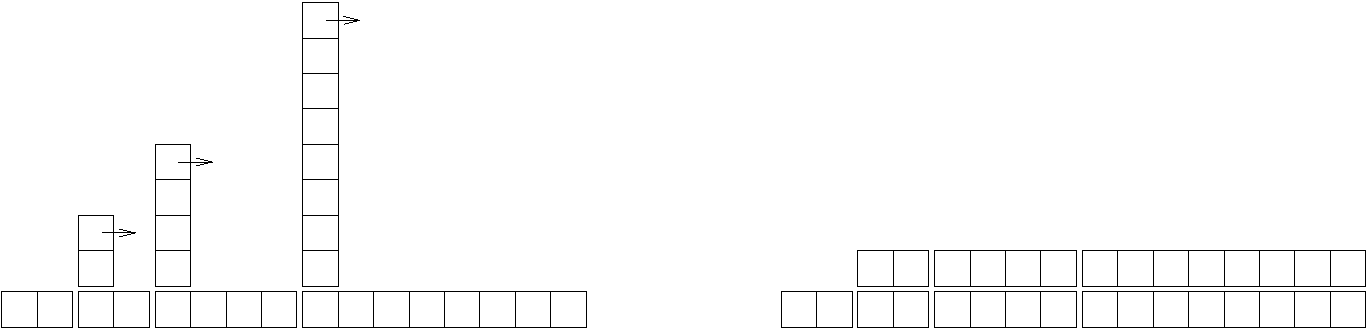
\includegraphics[width=5.5in]{figs/towers.pdf}}
\caption{The cost of a hashtable add.\label{fig.hash}}
\end{figure}

The extra work of rehashing appears as a sequence of increasingly
tall towers with increasing space between them.  Now if you knock
over the towers, spreading the cost of resizing over all
adds, you can see graphically that the total cost after $n$
adds is $2n - 2$.

An important feature of this algorithm is that when we resize the
HashTable it grows geometrically; that is, we multiply the size by a
constant.  If you increase the size
arithmetically---adding a fixed number each time---the average time
per {\tt add} is linear.
\index{geometric resizing}

You can download my implementation of HashMap from
\url{http://thinkpython2.com/code/Map.py}, but remember that there
is no reason to use it; if you want a map, just use a Python dictionary.

\section{Glossary}

\begin{description}

\item[analysis of algorithms:] A way to compare algorithms in terms of
their run time and/or space requirements.
\index{analysis of algorithms}

\item[machine model:] A simplified representation of a computer used
to describe algorithms.
\index{machine model}

\item[worst case:] The input that makes a given algorithm run slowest (or
require the most space.
\index{worst case}

\item[leading term:] In a polynomial, the term with the highest exponent.
\index{leading term}

\item[crossover point:] The problem size where two algorithms require
the same run time or space. 
\index{crossover point}

\item[order of growth:] A set of functions that all grow in a way
considered equivalent for purposes of analysis of algorithms. 
For example, all functions that grow linearly belong to the same
order of growth.
\index{order of growth}

\item[Big-Oh notation:] Notation for representing an order of growth;
for example, $O(n)$ represents the set of functions that grow
linearly. 
\index{Big-Oh notation}

\item[linear:] An algorithm whose run time is proportional to
problem size, at least for large problem sizes.
\index{linear}

\item[quadratic:] An algorithm whose run time is proportional to
$n^2$, where $n$ is a measure of problem size.
\index{quadratic}

\item[search:] The problem of locating an element of a collection
(like a list or dictionary) or determining that it is not present.
\index{search}

\item[hashtable:] A data structure that represents a collection of
key-value pairs and performs search in constant time.
\index{hashtable}

\end{description}


\chapter{The {\tt passdrill} utility}
\label{passdrill}

\index{passdrill}

This is a full listing of the {\tt passdrill} example. Its main goal is to check the Go syntax highlighting.

\lstinputlisting[language=Golang]{z/passdrill.go}



\printindex

\clearemptydoublepage
%\blankpage
%\blankpage
%\blankpage


\end{document}
